\documentclass[a4paper,10pt]{IEEEtran}

%% Language and font encodings
\usepackage[english,spanish,es-tabla]{babel}
\usepackage[utf8]{inputenc}
\usepackage[T1]{fontenc}
\usepackage{cite}
\usepackage{amsmath, amsthm, amssymb, amsfonts} 
\usepackage[mathscr]{eucal}
\usepackage{ulem} % subrayar, tachar
\usepackage{multirow, array} % para las tablas
\usepackage{float} % para tablas, usar [H]
\usepackage{graphicx} % graficos
\usepackage{longtable} 
\usepackage{hyperref} % Agregar enlaces \href
\usepackage{pdflscape} %hoja en horizontal
\usepackage{listings} %agregar codigo al documento
\usepackage{amsmath} %multiline, matrix

%ppppppppppppppppppppppppppppppppppppppppppppppppppppppppppppppppppppppppppppppp

%% Sets page size and margins
% Margenes segun formato IEEE
\usepackage[a4paper,top=1.7cm,bottom=1.7cm,left=1.6cm,right=1.6cm,marginparwidth= 1.5cm]{geometry}

\title{
    \Huge{Computación paralela y distribuida\\
    \Huge{Práctica 1}    
}}
\author{
\normalsize{
    Sebastian Guerrero Salinas \hspace{0.2cm} sebguerrerosal@unal.edu.co\\
    Juan Camilo Monterrosa Sanchez \hspace{0.2cm} jcmonterrosas@unal.edu.co\\
    Guiselle Tatiana Zambrano Penagos \hspace{0.2cm} gtzambranop@unal.edu.co\\
    Universidad Nacional de Colombia\\
    \normalsize{Bogotá, Colombia, Abril 2 de 2020}
    \vspace{-0.5cm}
}}


\begin{document}

\twocolumn[
\begin{@twocolumnfalse}
\vspace{-0.5cm}
\maketitle

\begin{abstract}
\footnotesize{
El presente es el reporte de la primera práctica en la asignatura “Computación
paralela y distribuida”, práctica que consiste en la implementación y
comparación del rendimiento de un algoritmo que genere un efecto borroso sobre
una imagen. Este algoritmo se ejecutará en dos escenarios distintos con sus
respectivas instrucciones, y sobre cada uno de ellos se realizarán las pruebas
pertinentes con su respectivo informe de resultados.\\

\textbf{Palabras clave:} Efecto borroso, hilos, imagen, paralelización, tiempos
de respuesta.}
\end{abstract}

\end{@twocolumnfalse}
]

\small

\section{Introducci\'on}
Este documento es ofrece una comparación clara y concluyente del rendimiento de
un algoritmo para la generaci\'on del efecto borroso en una imagen en
escenarios diferidos uno del otro por las condiciones de paralelizaci\'on, el
primero de ellos en una ejecuci\'on secuencial y el segundo en una ejecuci\'on
con diferentes cantidades de hilos POSIX. Cada uno de los escenarios de
ejecuci\'on se probar\'a con tres tipos de im\'agenes y el algoritmo de
generaci\'on de efecto borroso ser\'a el mismo, una vez ejecutado cada
escenario se tendr\'a una imagen resultante de la aplicaci\'on del efecto y se
realizar\'a la toma de medidas de tiempo de respuesta para cada imagen y se
llevar\'a el registro de las mismas.

\section{Procedimiento} 
\begin{enumerate}
    \item \textit{Elaboraci\'on y prueba del algoritmo:}  \\ \\
    Para la construcci\'on del algoritmo generador del efecto borroso se tom\'o
    como base varias implementaciones del algoritmo “Fastest Gaussian blur” [1],
    en esta interpretaci\'on se defin\'ia el efecto Gaussian Blur de una
    funci\'on en dos dimensiones como la convoluci\'on de esa funci\'on con
    funciones Gaussianas en dos dimensiones. En este caso particular de la
    funci\'on Gaussiana adaptada se maneja una integral que est\'a \'unicamente
    definida por un par\'ametro $\sigma$ llamado desviaci\'on estándar y que para
    fines prácticos de comprensión del algoritmo lo notan como “radio”. Teniendo
    un caso discreto finito presentan las funciones en dos dimensiones como
    matrices de valores y se computa el volumen (integral) como una suma, como la
    funci\'on Gaussiana tiene valores muy cercanos a cero en ciertos radios, se
    usar\'an solo los valores $- r\leq x\leq r$, $- r\leq y \leq r$, es ac\'a
    donde se empieza a manejar el kernel, interpretado como la parte “\'util” del
    peso. As\'i el valor de convoluci\'on en la posici\'on $[i, j]$ es el
    promedio ponderado, es decir, la suma de los valores de la funci\'on
    alrededor de $[i, j]$ multiplicado por el peso. \\
    
    En el desarrollo de este reporte se decidi\'o estudiar y adaptar una de las 4
    implementaciones del “Fastest Gaussian blur”, m\'as espec\'ificamente la
    llamada “gaussBlur\_3” por el autor. Esta implementaci\'on define dos grandes funciones que terminan produciendo un “desenfoque unidimensional”, desenfoque el cual se describe como un desenfoque de caja y permite visualizar de mejor manera que las dos grandes funciones que lo producen tienen una complejidad de $O(n * r)$, complejidad heredada de dicho desenfoque de caja.\\
    
    El programa funciona dividiendo la imagen en los canales que la conforman, para este caso particular en el que nos encontramos trabajando sobre extensiones \textbf{.jpg} y \textbf{.jpeg}, se tienen los canales \textbf{R}, \textbf{G} y \textbf{B}, los cuales de manera secuencial son ingresados individualmente a la funci\'on generadora del algoritmo de \textbf{Blur}, ahora bien, para lograr la paralelizaci\'on, se opt\'o por repartir los datos de tal manera que las funciones correspondientes que modifican la informaci\'on de cada canal dividieran el proceso por la cantidad de hilos creados, utilizando as\'i una
    \textbf{Distribuci\'on de datos} de tipo \textbf{BlockWise}, como se representa a continuaci\'on: \\
    
    %Imagen del blockwise
    \begin{figure}[H]
        \centering
        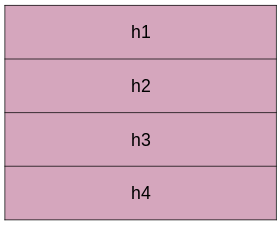
\includegraphics[scale = 0.5]{images/f00.png}
        \caption{Block-wise}
        \label{F00}
    \end{figure}{}
    
    \item \textit{Construcci\'on del programa secuencial:} \\ 

    Al analizar el problema buscando la mejor soluci\'on se logr\'o dar con una librer\'ia de manejo de imágenes con soporte y buena documentaci\'on para el lenguaje de programación a utilizar el cual es \textbf{C}, la librer\'ia en menci\'on es \textbf{STB} [2] y para poder hacer uso de la misma se deb\'ia descargar en el mismo directorio donde se tuviera el programa. En cuanto a la
    estructura del programa se decidi\'o empezar con la inclusi\'on de las librer\'ias que fueron m\'as exactamente 7, seguido de ello se incluye una macro de utilidad para verificaci\'on de errores, luego se define una estructura y varias funciones de comparaci\'on entre n\'umeros, le siguen funciones de manejo de im\'agenes y posterior a ello todas las funciones que componen el algoritmo de efecto borroso; para el \textit{main} del c\'odigo se dispondr\'a de sentencias que asemejan a un programa paralelizado con hilos POSIX pero para la disposici\'on particular de este programa en forma secuencial solo se manejar\'a con un hilo, lo cual refleja un comportamiento
    id\'oneo para este escenario. La organizaci\'on del \textit{main} consta de una verificaci\'on inicial de errores para el comando que ejecute el programa, seguido se encuentra la asignaci\'on del n\'umero de hilos, luego recibe el n\'umero que indica el tamaño del kernel, posteriormente se carga la imagen y le siguen las sentencias de manejo de hilos que, para el caso de
    este programa ser\'ia \'unicamente uno, finalmente termina guardando la imagen resultante y liberando la memoria de esta. \\
    
    \item \textit{Construcci\'on del programa con hilos POSIX:} \\ \\
    La estructura del escenario de paralelizaci\'on con hilos POSIX es en gran medida muy similar a la estructura del programa para el escenario secuencial ya que la estrategia de construcci\'on del mismo fue hacer un mismo estilo de programa que funcionara para ambos casos con la diferencia que para el caso de la paralelizaci\'on se var\'ia el n\'umero de hilos a ejecutar el programa y en el secuencial se deja este n\'umero constante con un valor de 1. \\
    
    \item \textit{Creaci\'on del script de ejecuci\'on total} \\ \\
    Como herramienta para la ejecuci\'on y prueba de los programas en este reporte se solicit\'o la construcci\'on de un script de ejecución total, es decir, un archivo de texto cuyo contenido es un conjunto de l\'ineas de comando, las cuales son ejecutadas de forma secuencial de principio a fin como si se estuvieran realizando de forma manual en la terminal de consola del sistema operativo que para este reporte es uno basado en Linux, más
    espec\'ificamente \textbf{Ubuntu 18.4}. \\

    El script creado y utilizado para esta ocasi\'on es llamado
    \textbf{“script\_ejecutar\_todo.sh”} y est\'a totalmente enfocado a la compilaci\'on y ejecuci\'on de los programas a evaluar, a la variaci\'on de los par\'ametros de ejecuci\'on de cada uno y la recolecci\'on de resultados de tiempo de cada uno en archivos de texto plano. La estructura del script se resume a continuación:
    
    \begin{enumerate}
        \item \textit{Compilaci\'on del programa:} dos l\'ineas de comandos que cumplir\'an la funci\'on de compilar los programas a evaluar, estas l\'ineas con los respectivos par\'ametros de funcionamiento de las librer\'ias que se usan en los archivos y la especificaci\'on del nombre
        del ejecutable. \\
        
        \item \textit{Resultados del programa en secuencial:} esta parte del script comienza con la creaci\'on del archivo llamado \textbf{“resultados.txt”} el cual ser\'a el archivo donde se colectar\'an los resultados. Seguido de eso, comienza la parte del registro de datos para el programa que trabaja de forma secuencial, se realiza con caracteres sencillos una figura de tabla con encabezado que dice
        \textbf{“Ejecución secuencial”}, seguido de ello se indica el valor inicial del kernel que ser\'a de 3, luego, un separador que indica que se mostrar\'an los resultados de la primera imagen, la imagen de 720p, despu\'es un condicional que indicar\'a el tama\~no de kernel con el que se est\'a trabajando en el archivo de resultados seguido de la l\'inea de comando que ejecuta el programa especificando el nombre del ejecutable y la imagen que va a tratar el programa y toma el tiempo de dicha ejecuci\'on, finaliza esta parte con un incremento en el n\'umero de kernel en 2, todas las instrucciones del condicional est\'an destinadas a repetirse mientras el kernel no supere el valor de 15; todas estas
        instrucciones se repiten para las im\'agenes de 1080p y 4k
        respectivamente. \\
        
        \item \textit{Resultados del programa en paralelo:} esta parte del script comienza con la parte del registro de datos para el programa que trabaja de forma paralela con hilos POSIX, los datos ac\'a registrados ir\'an de igual manera al archivo \textbf{“resultados.txt”}, se realiza con caracteres sencillos una figura de tabla con encabezado que dice \textbf{“Ejecuci\'on en paralelo”}, seguido de ello se indica el valor inicial del kernel que ser\'a de 3 y el valor inicial de cantidad de hilos que ser\'a de 2, luego, un separador que indica que se mostrar\'an los resultados de la primera imagen, la imagen de 720p, despu\'es dos
        condicionales, uno dentro del otro con el prop\'osito de ir aumentando el tama\~no de kernel para el condicional externo e ir aumentando la cantidad de hilos para el condicional interno, sus instrucciones son indicar y grabar en el archivo de resultados el tama\~no de kernel y la cantidad de hilos con las que se ejecuta el programa cada vez, le sigue
        la l\'inea de comando que ejecuta el programa especificando el nombre del ejecutable y la imagen que va a tratar el programa y toma el tiempo de dicha ejecuci\'on, finaliza esta parte con un incremento en el n\'umero de kernel en 2 y multiplicando la cantidad de hilos por 2, todas las instrucciones de los condicionales est\'an destinadas a repetirse mientras el kernel no supere el valor de 15 y la cantidad de hilos se mantenga menor a 17; todas estas instrucciones se repiten para las im\'agenes de 1080p y 4k respectivamente.
    \end{enumerate}
\end{enumerate}

\section{Resultados}

%info del pc de Juan
El computador utilizado para realizar la ejecuci\'on de la pr\'actica y todas las pruebas cuenta con un procesador AMD A8 - 7410 con 2.2 GHz, tiene una memoria RAM de 4GB y un disco duro con una capacidad de 500GB.

Para obtener los datos, fue necesario ejecutar 10 veces el script llamado \textit{script\_ejecutar\_todo.sh} y los valores arrojados por este fueron manejados en un notebook en Colab \cite{01} en donde fueron promediados y clasificados de la siguiente manera:


\begin{itemize}
    \item \textbf{Kernel 3} 
        \begin{figure}[H]
            \centering
            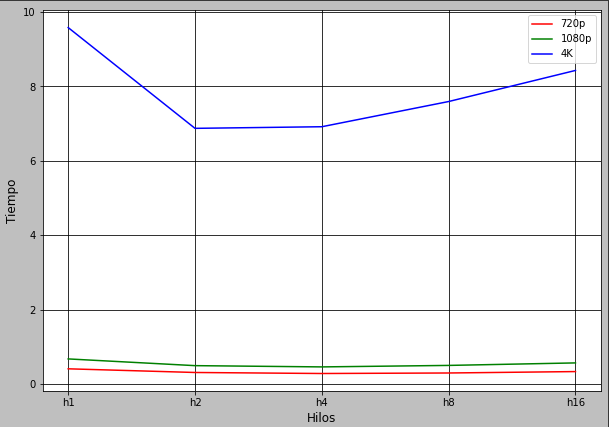
\includegraphics[scale = 0.3]{images/k3.png}
            \caption{Tiempo vs Hilos}
            \label{f00}
        \end{figure}{}
        
        \begin{figure}[H]
            \centering
            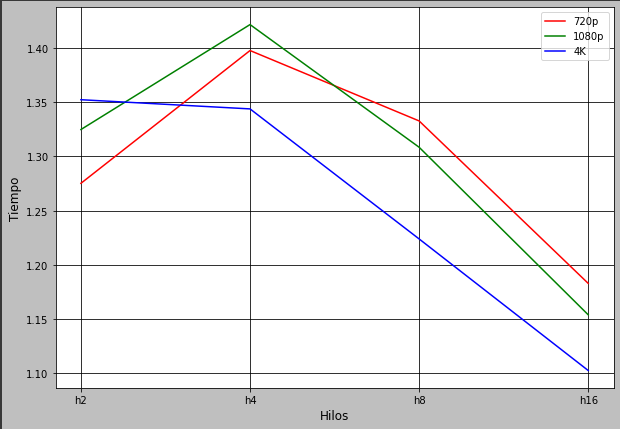
\includegraphics[scale = 0.3]{images/k3s.png}
            \caption{Speed-up}
            \label{f00a}
        \end{figure}{}
        
    \item \textbf{Kernel 5} 
        \begin{figure}[H]
            \centering
            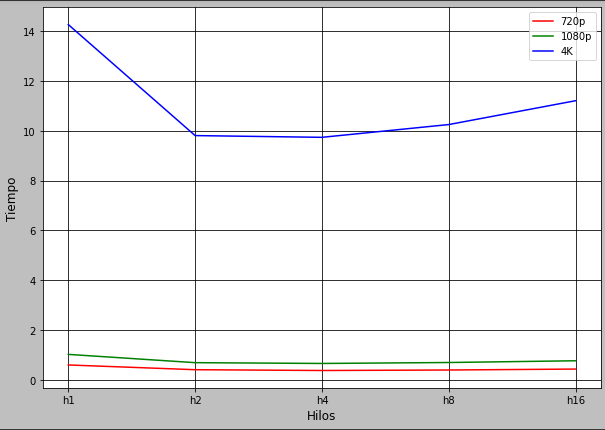
\includegraphics[scale = 0.3]{images/k5.png}
            \caption{Tiempo vs Hilos}
            \label{f01}
        \end{figure}{}
        
        \begin{figure}[H]
            \centering
            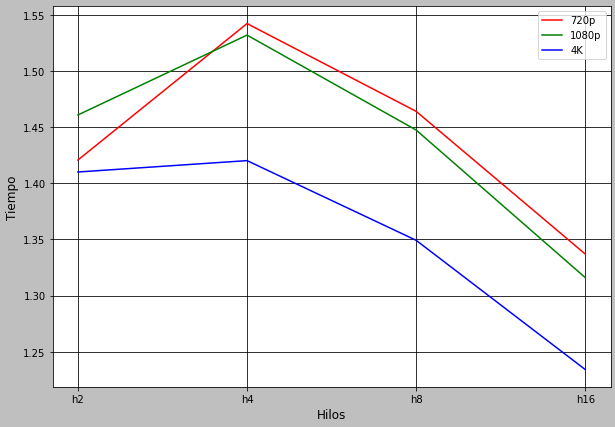
\includegraphics[scale = 0.3]{images/k5s.png}
            \caption{Speed-up}
            \label{f01a}
        \end{figure}{}
        
    \item \textbf{Kernel 7} 
        \begin{figure}[H]
            \centering
            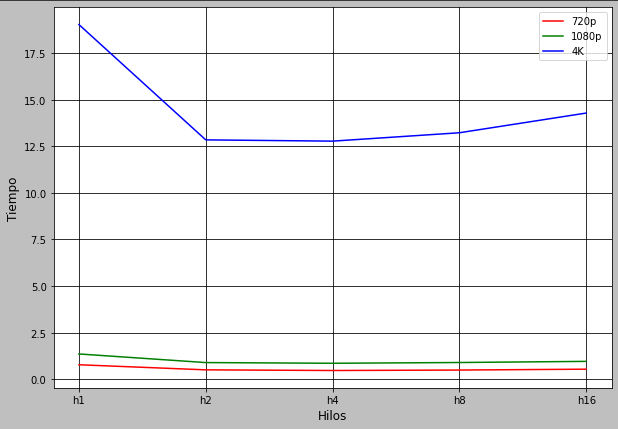
\includegraphics[scale = 0.3]{images/k7.png}
            \caption{Tiempo vs Hilos}
            \label{f02}
        \end{figure}{}
        
        \begin{figure}[H]
            \centering
            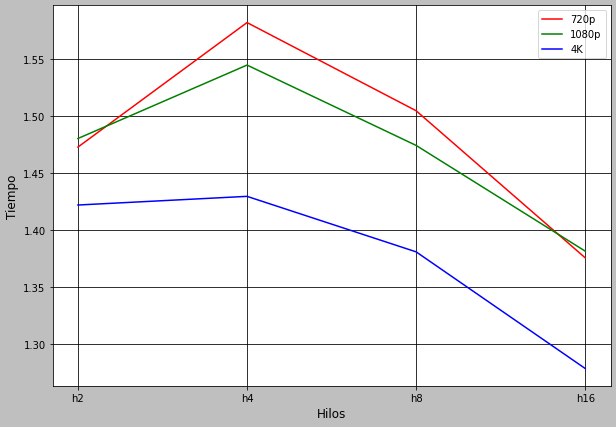
\includegraphics[scale = 0.3]{images/k7s.png}
            \caption{Speed-up}
            \label{f02a}
        \end{figure}{}
        
    \item \textbf{Kernel 9} 
        \begin{figure}[H]
            \centering
            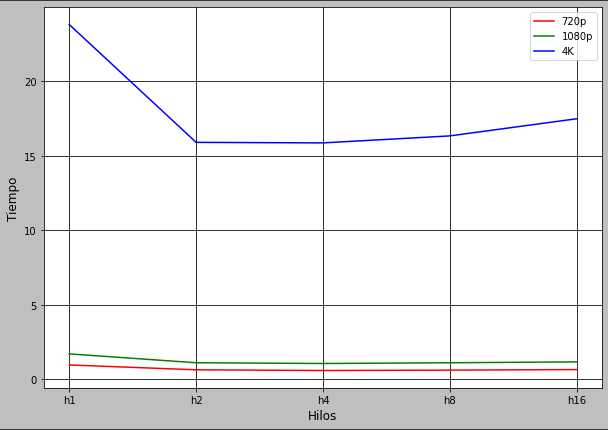
\includegraphics[scale = 0.3]{images/k9.png}
            \caption{Tiempo vs Hilos}
            \label{f03}
        \end{figure}{}
        
        \begin{figure}[H]
            \centering
            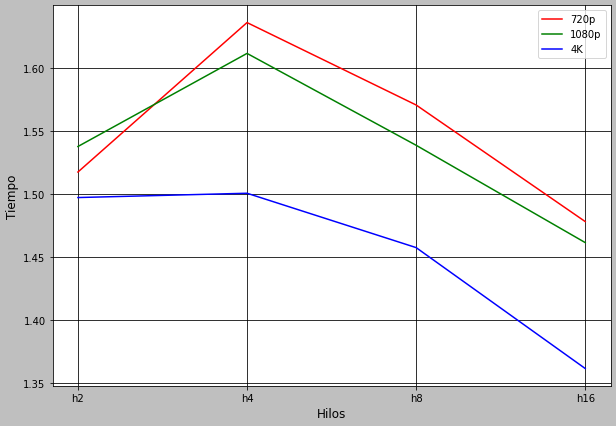
\includegraphics[scale = 0.3]{images/k9s.png}
            \caption{Speed-up}
            \label{f03a}
        \end{figure}{}
        
    \item \textbf{Kernel 11} 
        \begin{figure}[H]
            \centering
            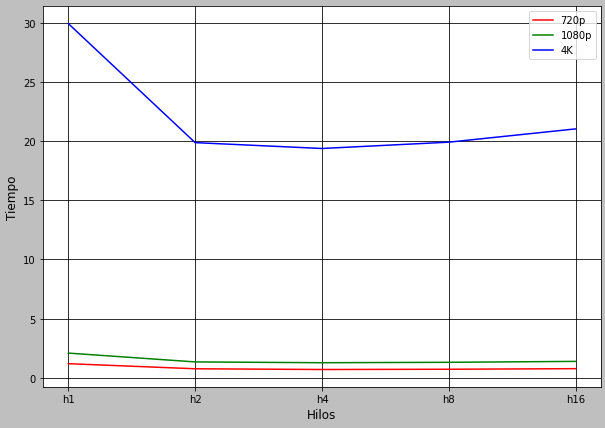
\includegraphics[scale = 0.3]{images/kB.png}
            \caption{Tiempo vs Hilos}
            \label{f04}
        \end{figure}{}
        
        \begin{figure}[H]
            \centering
            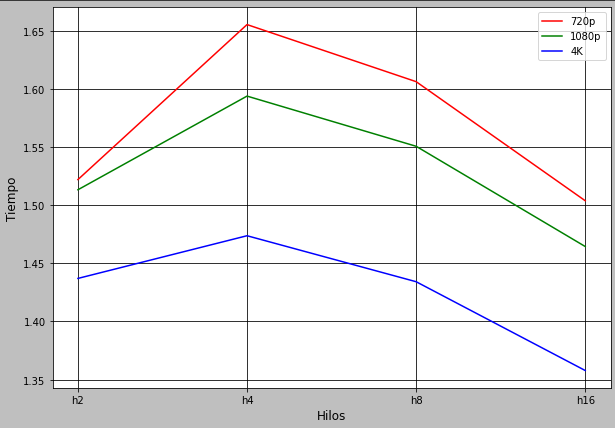
\includegraphics[scale = 0.3]{images/kBs.png}
            \caption{Speed-up}
            \label{f04a}
        \end{figure}{}
        
    \item \textbf{Kernel 13} 
        \begin{figure}[H]
            \centering
            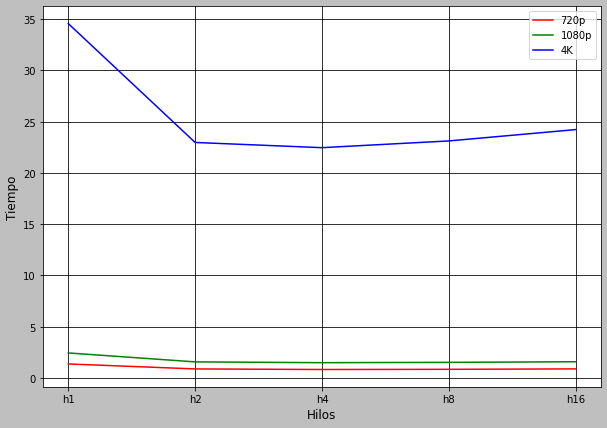
\includegraphics[scale = 0.3]{images/kD.png}
            \caption{Tiempo vs Hilos}
            \label{f05}
        \end{figure}{}
        
        \begin{figure}[H]
            \centering
            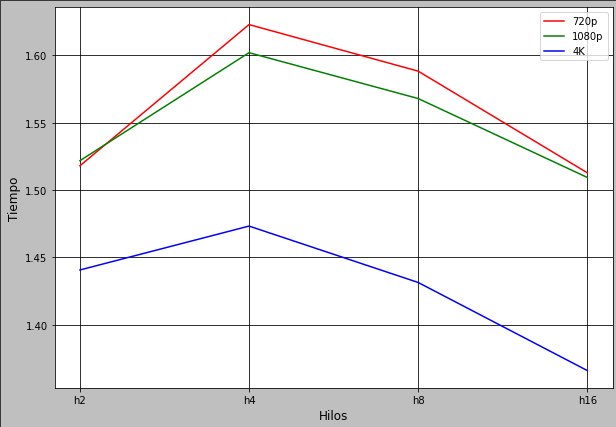
\includegraphics[scale = 0.3]{images/kDs.png}
            \caption{Speed-up}
            \label{f05a}
        \end{figure}{}
        
    \item \textbf{Kernel 15} 
        \begin{figure}[H]
            \centering
            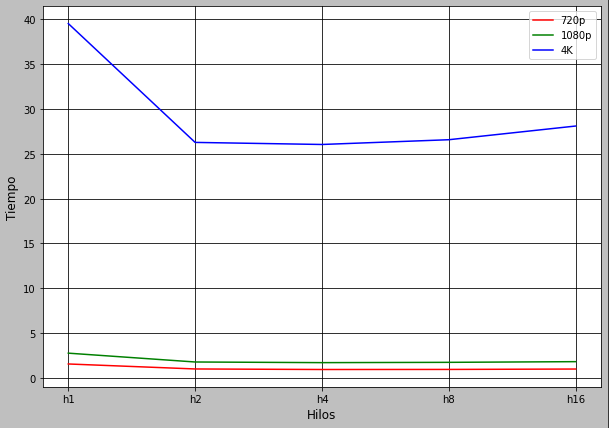
\includegraphics[scale = 0.3]{images/kF.png}
            \caption{Tiempo vs Hilos}
            \label{f06}
        \end{figure}{}
        
        \begin{figure}[H]
            \centering
            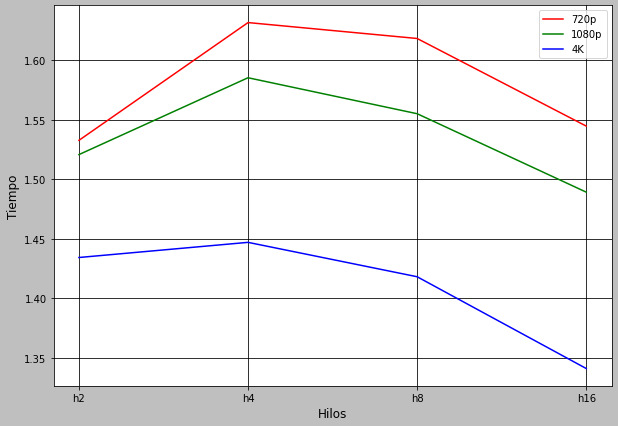
\includegraphics[scale = 0.3]{images/kFs.png}
            \caption{Speed-up}
            \label{f06a}
        \end{figure}{}
\end{itemize}{}

\section{Conclusiones}

\begin{itemize}
    \item Al incrementar el tamaño del kernel el efecto blur es más notable en las im\'agenes 
    \item A causa de la cantidad de píxeles, con n\'umeros de kernel grandes y bastantes hilos, la calidad del efecto borroso disminuye notoriamente
    \item \'Unicamente la imagen de 4k amerita realmente incrementar el tama\~no del kernel y aumentar los hilos ya que resalta m\'as la optimizaci\'on de tiempo de ejecuci\'on del programa
    \item Mediante el \textit{Speed-up} podemos notar el efecto que tienen los n\'uucleos de procesamiento de un computador en la programaci\'on paralela, puesto que en todas las diferentes ejecuciones variando los \textit{kernels} y la cantidad de hilos utilizados, el m\'aximo \textit{Speed-up} es 4, que resulta ser igual al n\'uumero de n\'ucleos del computador donde se esta ejecutando el programa. 
\end{itemize}{}


\begin{thebibliography}{50}
\scriptsize{

\bibitem{00} Fastest Gaussian Blur (in linear time). Available at:
\url{http://blog.ivank.net/fastest-gaussian-blur.html} \url{https://github.com}
\bibitem{01} Notebook Colab. Available at:
\url{https://colab.research.google.com/drive/1WvBwBzceWoZUzsvXcfuIBtCEchWDNFA6}

}
\end{thebibliography}{}

\end{document}
